
\section{Architecture Integration}

\subsection{Model Support}

\begin{table}[H]
\centering
\small
\begin{tabular}{lllll}
\toprule
\textbf{Architecture} & \textbf{Attention class} & \textbf{RoPE?} & \textbf{GQA?} & \textbf{Verified} \\
\midrule
DistilBERT & \texttt{MultiHeadSelfAttention} \& No \& No &  \\
RoBERTa & \texttt{BertSelfAttention} \& No \& No &  \\
GPT-2 & \texttt{GPT2Attention} \& No \& No &  \\
Qwen3.5 & \texttt{Qwen3Attention} \& Yes \& Yes \& not tested \\
\bottomrule
\end{tabular}
\end{table}

\subsection{Weight Transfer}

\subsubsection{DistilBERT (Flat)}

\begin{lstlisting}
q\_lin: Linear(768, 768)
k\_lin: Linear(768, 768)
v\_lin: Linear(768, 768)
out\_lin: Linear(768, 768)
\end{lstlisting}

\textbf{Copy:} Direct. \texttt{is\_nested\_encoder = False}.

\subsubsection{RoBERTa (Nested)}

\begin{lstlisting}
attention.self.query: Linear(768, 768)
attention.self.key: Linear(768, 768)
attention.self.value: Linear(768, 768)
attention.output.dense: Linear(768, 768)
\end{lstlisting}

\textbf{Copy:} Extract from inner \texttt{self}. \texttt{is\_nested\_encoder = True}, skip own 
\texttt{out\_proj}.

\subsubsection{GPT-2 (Causal)}

\begin{lstlisting}
attn.c\_attn: Conv1D(768, 2304)   # fused Q, K, V
attn.c\_proj: Conv1D(768, 768)
\end{lstlisting}

\textbf{Copy:} Transpose and split. Direct for \texttt{c\_proj}.

\subsubsection{Qwen3.5 (GQA + RoPE)}

\begin{lstlisting}
q\_proj: Linear(1024, 2048)   # 8 heads $\times$ 256
k\_proj: Linear(1024, 512)    # 2 heads $\times$ 256
v\_proj: Linear(1024, 512)
o\_proj: Linear(2048, 1024)
\end{lstlisting}

\textbf{Copy:} Direct, then \texttt{repeat\_kv} at runtime. RoPE applied to landmarks 
implicitly via the pooled $Q, K$ (see  5.5).

\subsection{Injection Algorithm}

\textbf{Algorithm 2:} Inject Primal Attention into a full model
\begin{lstlisting}
Input:  model M, config c, m (landmark count)
Output: M with Primal attention

1:  for   in transformer\_layers(M) do
2:      src $\leftarrow$ extract\_attention( )
3:      if src is None: continue
4:      new $\leftarrow$ PrimalAttention(config=c, pretrained\_attn=src)
5:      replace\_attention( , new)
6: end for
\end{lstlisting}

\subsection{Handling RoPE}

RoPE is applied to $Q, K$ \textbf{before} landmark pooling. This preserves the 
relative positions of the landmark summaries.

\begin{lstlisting}
Q, K = apply\_rotary\_pos\_emb(Q, K, cos, sin, position\_ids)
Q\_land, K\_land = pool\_to\_landmarks(Q, K, m)
\end{lstlisting}

\subsection{Handling GQA}

For grouped-query attention, we repeat KV heads \textbf{before} pooling:

\begin{lstlisting}
if num\_kv\_heads \textless{} num\_heads:
    K = repeat\_kv(K, num\_heads // num\_kv\_heads)
    V = repeat\_kv(V, num\_heads // num\_kv\_heads)
\end{lstlisting}

Then landmarks are computed on the repeated KV.

\subsection{Causality}

For decoder models, causal masking is applied to the \textbf{approximate} attention 
matrix:

\begin{lstlisting}
causal\_mask = torch.triu(torch.full((L, L), -1e4), diagonal=1)
attn = attn + causal\_mask
\end{lstlisting}

\textbf{Note.} This is not a true causal approximation (landmarks see all tokens), 
but empirically works for generation. See  8.5 for analysis.

\subsection{Failure Handling}

\texttt{inject\_primal} returns \texttt{None} on failure and logs the error:

\begin{lstlisting}
try:
    new\_attn = PrimalAttention(config=config, pretrained\_attn=target, **kwargs)
except Exception:
    raise RuntimeError("copy\_weights failed")
\end{lstlisting}

The outer loop can catch this and continue with the next layer.

\subsection{Parameter Count}

Primal Attention has the \textbf{same parameter count} as MHA:

\begin{table}[H]
\centering
\small
\begin{tabular}{ll}
\toprule
\textbf{Projection} & \textbf{Params} \\
\midrule
$W_Q$ & $d \cdot H d_h$ \\
$W_K$ & $d \cdot H_{kv} d_h$ \\
$W_V$ & $d \cdot H_{kv} d_h$ \\
$W_O$ & $H d_h \cdot d$ \\
\bottomrule
\end{tabular}
\end{table}

With LoRA recovery at rank $r_L$, add $2 r_L (d + d_h H)$ per projection.

\subsection{Registry}

\begin{lstlisting}
@ATTENTION\_REGISTRY.register("primal")
@ATTENTION\_REGISTRY.register("primal\_attention")
class PrimalAttention(BaseAttention): ...
\end{lstlisting}

\subsection{Failure Modes}

\begin{lstlisting}

---
\end{lstlisting}

\begin{figure}[H]
\centering
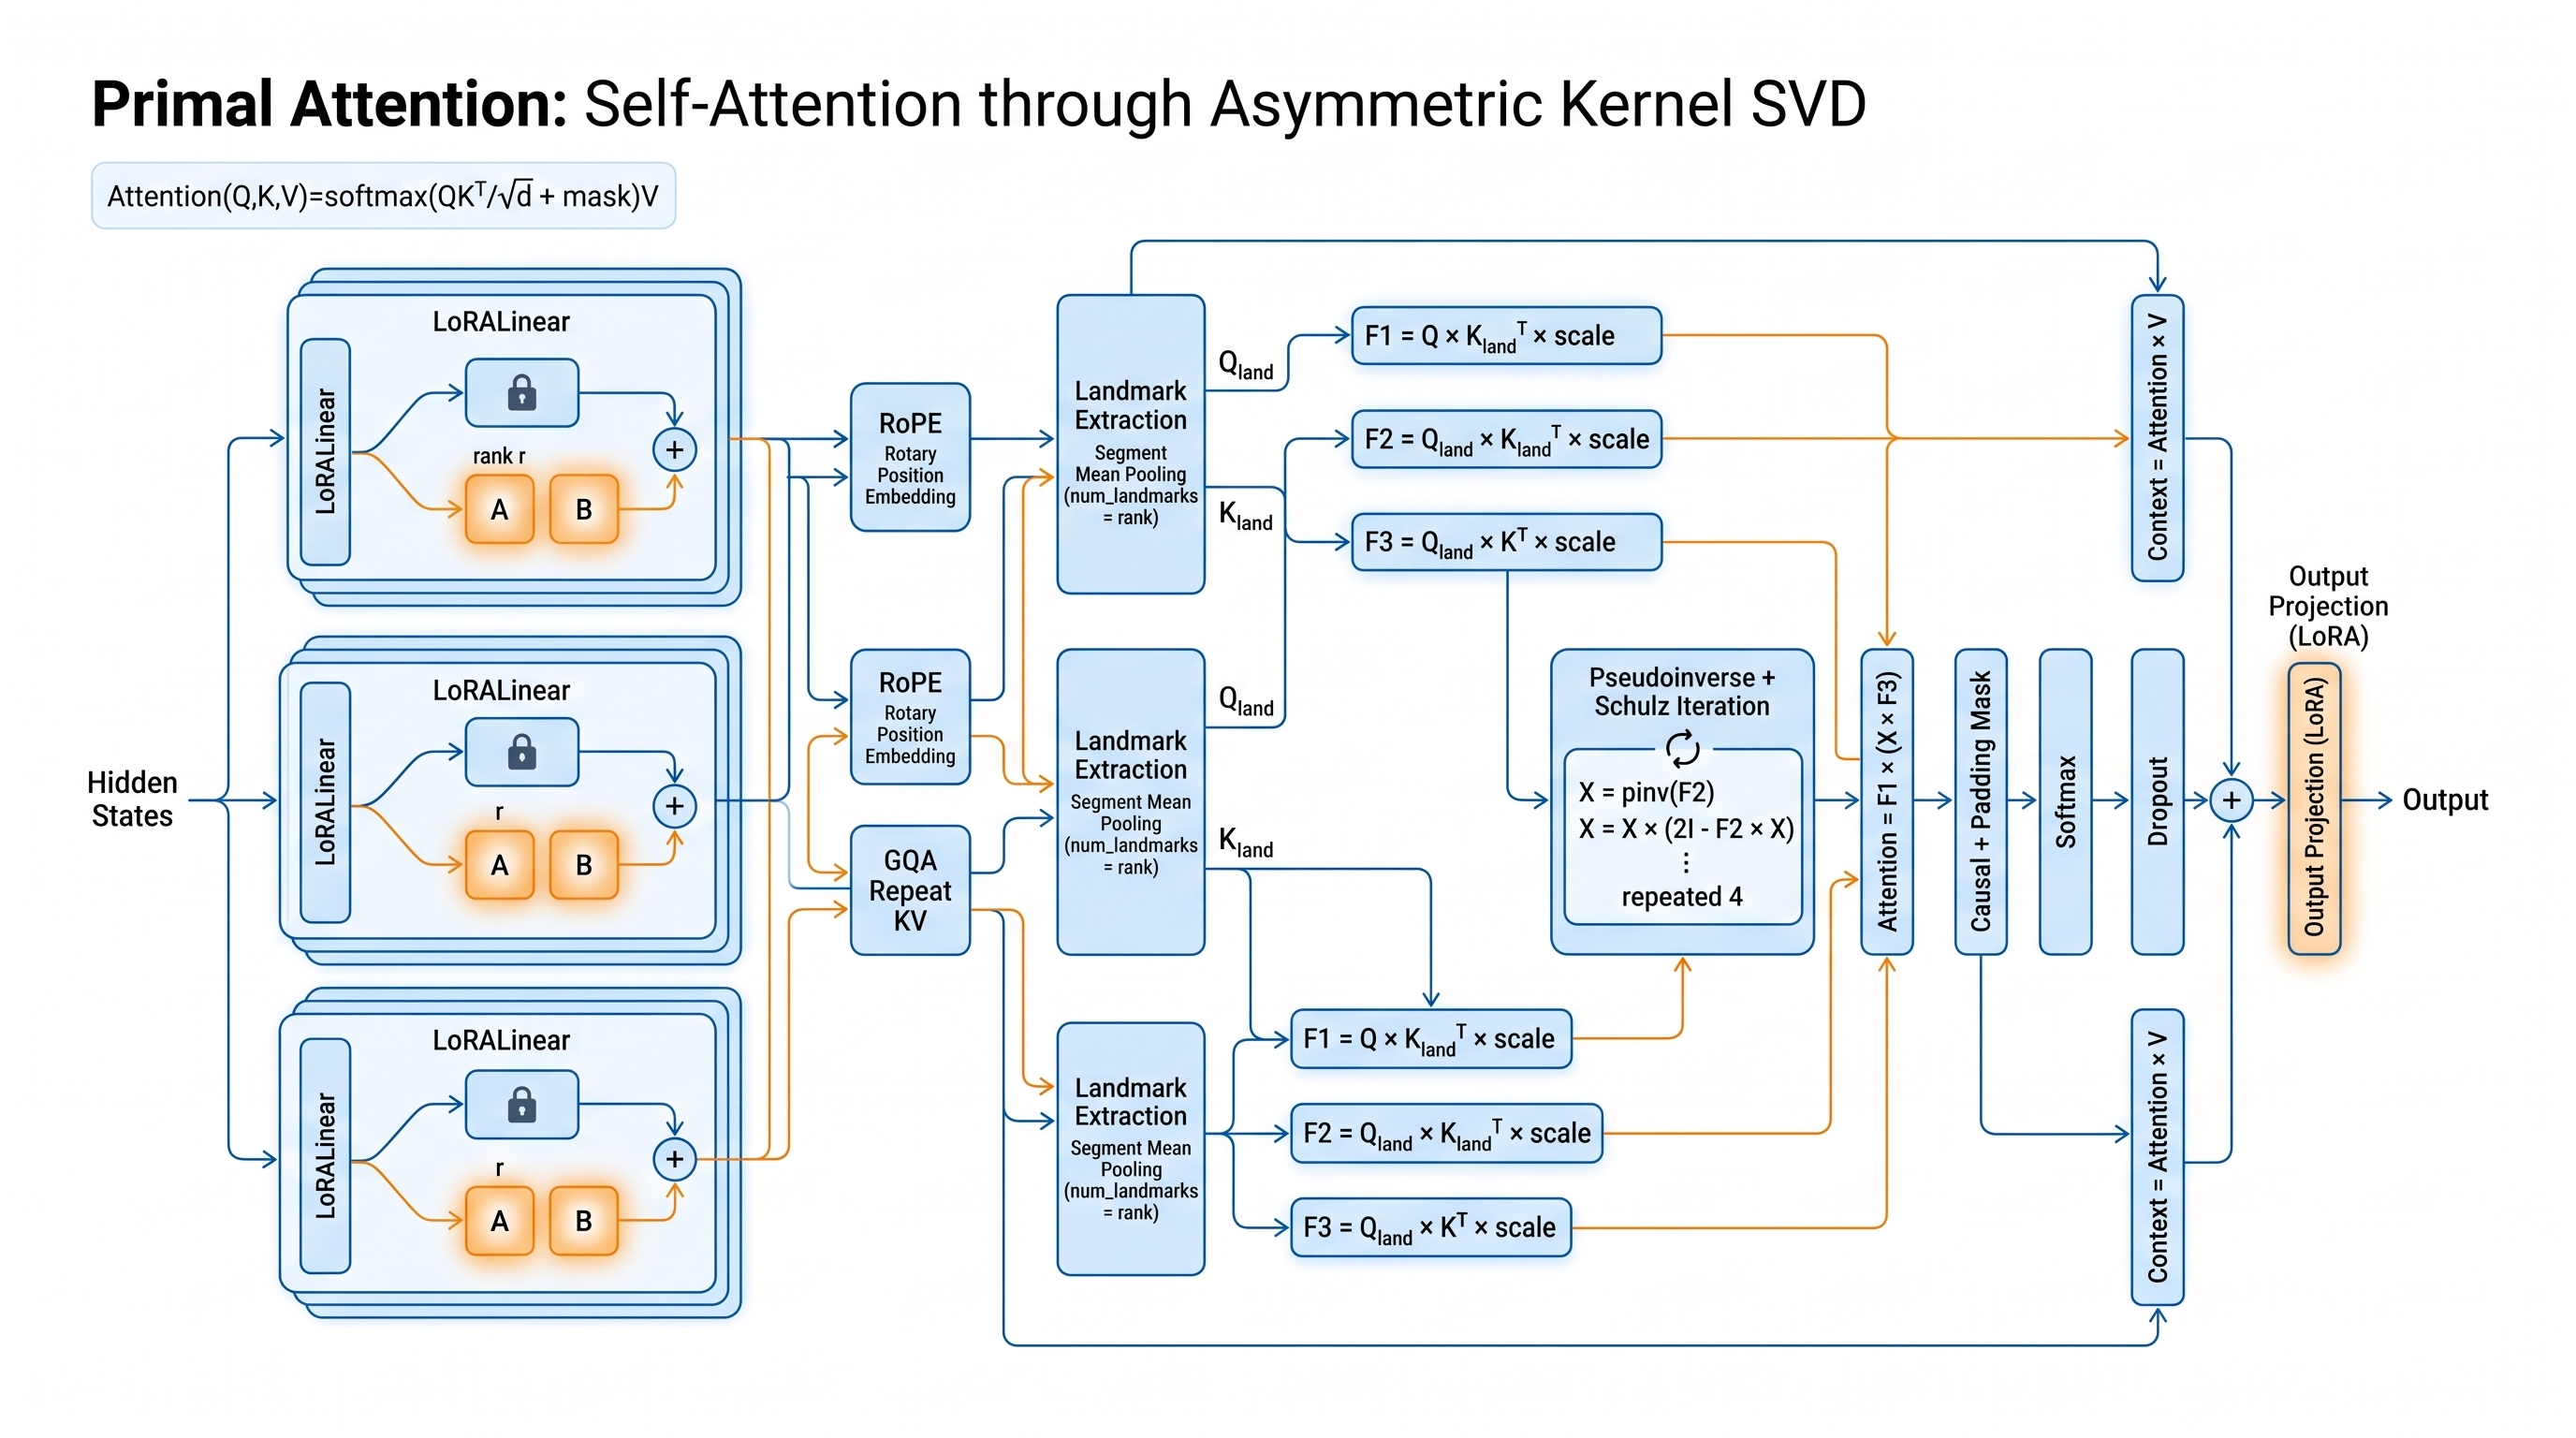
\includegraphics[width=\linewidth]{figures/architecture.jpeg}
\caption{High-level architectural diagram of Primal.}
\label{fig:arch_Primal}
\end{figure}

